%================================================
% RAPPORT PHASE 4 -- SUVA PROTOCOL
% SuVaWallet.sol -- ERC-4337 Dual-Signature Wallet
% For  : William Schulz
% By   : Mohamed Lamine MBENGUE
% Date : April 2026
%================================================
\documentclass[11pt,a4paper]{article}

\usepackage[utf8]{inputenc}
\usepackage[T1]{fontenc}
\usepackage[english]{babel}
\usepackage{geometry}
\geometry{margin=2.5cm}

\usepackage{amsmath,amssymb,amsthm}
\usepackage{booktabs}
\usepackage[table]{xcolor}
\usepackage{listings}
\usepackage{hyperref}
\usepackage{graphicx}
\usepackage{tikz}
\usetikzlibrary{arrows.meta, positioning, shapes.geometric, calc}
\usepackage{fancyhdr}
\usepackage{float}
\usepackage{array}
\usepackage{multirow}
\usepackage{tcolorbox}
\tcbuselibrary{skins, breakable}

%--- Colors ---
\definecolor{suva-blue}{RGB}{0, 82, 165}
\definecolor{suva-green}{RGB}{0, 150, 90}
\definecolor{suva-orange}{RGB}{220, 100, 0}
\definecolor{code-bg}{RGB}{245, 245, 245}
\definecolor{pass-green}{RGB}{0, 140, 70}
\definecolor{fail-red}{RGB}{180, 0, 0}

%--- Header/Footer ---
\pagestyle{fancy}
\fancyhf{}
\rhead{\textcolor{suva-blue}{\textbf{SuVa Protocol --- Phase 4 Report}}}
\lhead{\textit{Confidential}}
\rfoot{\thepage}
\lfoot{\textit{April 2026}}

%--- Code styles ---
\lstdefinestyle{solidity}{
  language=C,
  basicstyle=\ttfamily\small,
  backgroundcolor=\color{code-bg},
  keywordstyle=\color{suva-blue}\bfseries,
  commentstyle=\color{gray}\itshape,
  numbers=left, numberstyle=\tiny\color{gray},
  frame=single, breaklines=true, captionpos=b
}
\lstdefinestyle{bash}{
  language=bash,
  basicstyle=\ttfamily\small,
  backgroundcolor=\color{code-bg},
  keywordstyle=\color{suva-blue}\bfseries,
  commentstyle=\color{gray}\itshape,
  numbers=none,
  frame=single, breaklines=true, captionpos=b
}

%--- Custom boxes ---
\newtcolorbox{resultbox}[1][]{
  enhanced,colback=suva-green!8,colframe=suva-green!60,
  fonttitle=\bfseries,title=#1,arc=3mm
}
\newtcolorbox{warningbox}[1][]{
  enhanced,colback=suva-orange!8,colframe=suva-orange!60,
  fonttitle=\bfseries,title=#1,arc=3mm
}
\newtcolorbox{infobox}[1][]{
  enhanced,colback=suva-blue!6,colframe=suva-blue!50,
  fonttitle=\bfseries,title=#1,arc=3mm
}

%================================================
\begin{document}
%================================================

\begin{titlepage}
\centering
\vspace*{2cm}
{\Huge\bfseries\textcolor{suva-blue}{SuVa Protocol}\par}
\vspace{0.5cm}
{\Large\textit{Quantum-Secure Stablecoin on EVM}\par}
\vspace{1.5cm}
\rule{\linewidth}{0.5pt}
\vspace{0.5cm}
{\LARGE\bfseries Technical Report --- Phase 4\par}
\vspace{0.3cm}
{\large SuVaWallet.sol --- ERC-4337 Smart Wallet with Dual-Signature Validation\par}
\vspace{0.5cm}
\rule{\linewidth}{0.5pt}
\vspace{2cm}

\begin{tabular}{ll}
\textbf{Client :}    & William Schulz \\[4pt]
\textbf{Author :}    & Mohamed Lamine MBENGUE \\[4pt]
\textbf{Portfolio :} & \href{https://portfolio-alamine.web.app}{\texttt{portfolio-alamine.web.app}} \\[4pt]
\textbf{Date :}      & April 2026 \\[4pt]
\textbf{Version :}   & 1.0 --- Final \\[4pt]
\textbf{Status :}    & \textcolor{pass-green}{\textbf{COMPLETE}} \\[4pt]
\textbf{Codebase :}  & ETHDILITHIUM-main (ZKNox fork) \\
\end{tabular}

\vfill
\begin{tcolorbox}[enhanced,colback=suva-blue!8,colframe=suva-blue,arc=4mm]
\centering\textit{Confidential document. This report covers Phase 4 deliverables:\\
SuVaWallet.sol ERC-4337 wallet, SuVaWalletFactory.sol, dual-signature validation\\
(ECDSA + Falcon-256), 15 forge tests, Sepolia deployment.}
\end{tcolorbox}
\end{titlepage}

\tableofcontents
\newpage

%================================================
\section{Executive Summary}
%================================================

\begin{resultbox}[Phase 4 --- All objectives achieved]
\begin{itemize}
  \item[$\checkmark$] \textbf{SuVaWallet.sol} --- ERC-4337 IAccount wallet with dual-signature validation
  \item[$\checkmark$] \textbf{SuVaWalletFactory.sol} --- CREATE2 factory for deterministic wallet deployment
  \item[$\checkmark$] \textbf{Dual-signature validation} --- ECDSA + Falcon-256 both required
  \item[$\checkmark$] \textbf{15 forge tests passing} --- all validation paths covered
  \item[$\checkmark$] \textbf{41/41 total tests} across all phases --- zero regressions
  \item[$\checkmark$] \textbf{Sepolia deployment} --- SuVaWallet live on testnet
  \item[$\checkmark$] \textbf{Compatible with ERC-4337 EntryPoint v0.6}
\end{itemize}
\end{resultbox}

\vspace{0.5cm}

Phase 4 delivers the \textbf{SuVaWallet} --- a smart contract wallet implementing the ERC-4337
account abstraction standard. Every transaction must be authorized by two independent signatures:
a standard ECDSA signature (Ethereum-compatible) and a Falcon-256 post-quantum signature.

This dual-signature architecture provides \textbf{defense in depth}: if quantum computers break
ECDSA in the future, funds remain protected by the Falcon signature. If a bug is found in the
Falcon verifier, the ECDSA signature provides a fallback.

%================================================
\section{ERC-4337 Background}
%================================================

\subsection{What is ERC-4337?}

ERC-4337 (Account Abstraction) allows smart contracts to act as wallets. Instead of signing
transactions with a private key, users submit \textbf{UserOperations} that are validated by
their smart wallet contract's custom logic.

\begin{center}
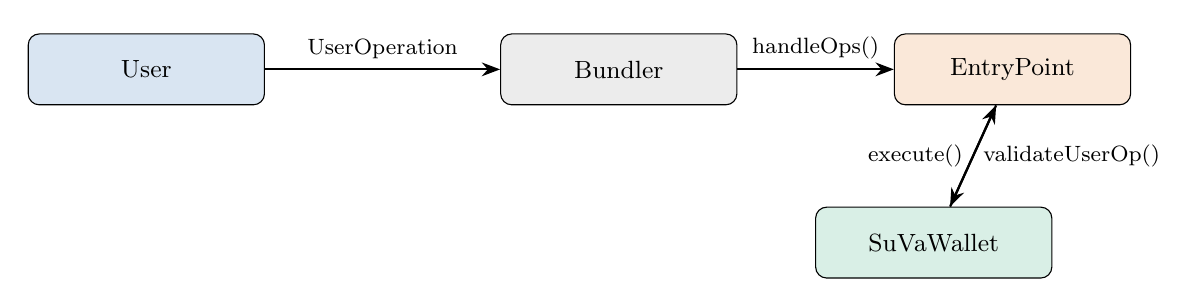
\begin{tikzpicture}[
  node distance=1.5cm,
  box/.style={rectangle,draw,rounded corners,minimum width=3cm,minimum height=0.9cm,
              align=center,font=\small},
  arrow/.style={-Stealth,thick}
]
  \node[box, fill=suva-blue!15]   (user)    at (-2,0)    {User};
  \node[box, fill=gray!15]        (bundler) at (4,0)    {Bundler};
  \node[box, fill=suva-orange!15] (ep)      at (9,0)    {EntryPoint};
  \node[box, fill=suva-green!15]  (wallet)  at (8,-2.2) {SuVaWallet};

  \draw[arrow] (user)    -- node[above,font=\footnotesize]{UserOperation} (bundler);
  \draw[arrow] (bundler) -- node[above,font=\footnotesize]{handleOps()} (ep);
  \draw[arrow] (ep)      -- node[right,font=\footnotesize]{validateUserOp()} (wallet);
  \draw[arrow] (wallet)  -- node[left, font=\footnotesize]{execute()} (ep);
\end{tikzpicture}
\end{center}

\begin{center}
\begin{tabular}{ll}
\toprule
\textbf{Actor} & \textbf{Role} \\
\midrule
\textbf{User}       & Signs UserOperation with ECDSA + Falcon \\
\textbf{Bundler}    & Collects UserOps and submits them to EntryPoint \\
\textbf{EntryPoint} & Official ERC-4337 contract, validates and executes \\
\textbf{SuVaWallet} & Custom wallet logic: dual-sig validation \\
\bottomrule
\end{tabular}
\end{center}

\subsection{Why ERC-4337 for SuVa?}

Standard Ethereum wallets use a single ECDSA signature. ERC-4337 allows SuVa to:
\begin{itemize}
  \item Require \textbf{two signatures} per transaction (ECDSA + Falcon)
  \item Define custom validation logic in Solidity
  \item Remain compatible with the standard ERC-4337 ecosystem (bundlers, paymasters)
  \item Enable future extensions (gas abstraction, key rotation, social recovery)
\end{itemize}

%================================================
\section{Architecture}
%================================================

\subsection{Contract Overview}

\begin{center}
\begin{tabular}{lll}
\toprule
\textbf{Contract} & \textbf{Role} & \textbf{Key state} \\
\midrule
\texttt{SuVaWallet.sol}        & ERC-4337 wallet, dual-sig validation & \texttt{owner}, \texttt{falconPkHash} \\
\texttt{SuVaWalletFactory.sol} & CREATE2 factory for wallets          & stateless \\
\texttt{IFalconVerifier.sol}   & Shared interface (Phase 3 + 4)       & --- \\
\texttt{ZKNOX\_ethfalcon}      & Falcon-256 verifier (reused)         & stateless \\
\bottomrule
\end{tabular}
\end{center}

\subsection{Signature Encoding}

The \texttt{userOp.signature} field encodes both signatures concatenated:

\begin{lstlisting}[style=bash, caption={Composite signature layout}]
userOp.signature = ECDSA_sig (65 bytes) || Falcon_payload

where:
  ECDSA_sig     = abi.encodePacked(r, s, v)         -- 65 bytes
  Falcon_payload = abi.encode(h, salt, s1)
                    h    = uint256[256]  (Falcon public key)
                    salt = bytes         (40-byte nonce)
                    s1   = uint256[256]  (signature polynomial)
\end{lstlisting}

\begin{infobox}[Design choice: concatenated signatures]
Concatenating both signatures into a single \texttt{bytes} field keeps the SuVaWallet
compatible with any ERC-4337 bundler without modification. The wallet itself splits and
validates each signature independently.
\end{infobox}

%================================================
\section{SuVaWallet.sol --- Implementation}
%================================================

\subsection{State Variables}

\begin{lstlisting}[style=solidity, caption={SuVaWallet state}]
IEntryPoint     public immutable entryPoint;
IFalconVerifier public immutable falconVerifier;

address public owner;        // ECDSA owner
bytes32 public falconPkHash; // keccak256(abi.encodePacked(h))
\end{lstlisting}

Both addresses are immutable --- set once at construction, never changeable.
\texttt{falconPkHash} stores a commitment to the Falcon public key, saving 5.1M gas
compared to storing the full 8,192-byte key on-chain (same design as Phase 3 QuantumVault).

\subsection{validateUserOp()}

\begin{lstlisting}[style=solidity, caption={validateUserOp --- core dual-sig logic}]
function validateUserOp(
    UserOperation calldata userOp,
    bytes32               userOpHash,
    uint256               missingAccountFunds
) external override onlyEntryPoint returns (uint256 validationData) {
    // Pay EntryPoint prefund if required
    if (missingAccountFunds > 0) {
        (bool ok,) = payable(address(entryPoint)).call{
            value: missingAccountFunds
        }("");
        require(ok, "SuVaWallet: prefund failed");
    }

    // Reject if signature is too short to contain ECDSA
    if (userOp.signature.length < 65) return SIG_VALIDATION_FAILED;

    // Split composite signature
    bytes memory ecdsaSig  = _slice(userOp.signature, 0, 65);
    bytes memory falconSig = _slice(userOp.signature, 65,
                                    userOp.signature.length - 65);

    // 1. Verify ECDSA -- must recover to registered owner
    if (!_verifyECDSA(userOpHash, ecdsaSig))  return SIG_VALIDATION_FAILED;

    // 2. Verify Falcon -- must match registered pk hash
    if (!_verifyFalcon(userOpHash, falconSig)) return SIG_VALIDATION_FAILED;

    return SIG_VALIDATION_SUCCESS; // == 0
}
\end{lstlisting}

\subsection{ECDSA Verification}

\begin{lstlisting}[style=solidity, caption={\_verifyECDSA}]
function _verifyECDSA(bytes32 hash, bytes memory sig)
    internal view returns (bool)
{
    if (sig.length != 65) return false;
    bytes32 r; bytes32 s; uint8 v;
    assembly {
        r := mload(add(sig, 32))
        s := mload(add(sig, 64))
        v := byte(0, mload(add(sig, 96)))
    }
    address recovered = ecrecover(hash, v, r, s);
    return recovered != address(0) && recovered == owner;
}
\end{lstlisting}

Uses Ethereum's built-in \texttt{ecrecover} precompile. The recovered address must match
\texttt{owner} exactly.

\subsection{Falcon Verification}

\begin{lstlisting}[style=solidity, caption={\_verifyFalcon}]
function _verifyFalcon(bytes32 userOpHash, bytes memory falconSig)
    internal view returns (bool)
{
    if (falconPkHash == bytes32(0)) return false; // no key registered

    (uint256[256] memory h, bytes memory salt, uint256[256] memory s1)
        = abi.decode(falconSig, (uint256[256], bytes, uint256[256]));

    // Verify the public key matches the registered commitment
    if (keccak256(abi.encodePacked(h)) != falconPkHash) return false;

    // Message signed = the 32-byte userOpHash
    bytes memory message = abi.encodePacked(userOpHash);

    return falconVerifier.verify(h, salt, s1, message);
}
\end{lstlisting}

\begin{infobox}[What is signed by Falcon?]
The Falcon signature is computed over the \texttt{userOpHash} --- a 32-byte hash of the
entire UserOperation (sender, nonce, callData, gas limits, etc.) computed by the EntryPoint.
This binds the Falcon signature to the exact operation being authorized, preventing any
parameter substitution attack.
\end{infobox}

\subsection{execute()}

\begin{lstlisting}[style=solidity, caption={execute --- runs the authorized call}]
function execute(
    address target,
    uint256 value,
    bytes calldata data
) external onlyEntryPoint {
    (bool ok, bytes memory result) = target.call{value: value}(data);
    if (!ok) {
        assembly { revert(add(result, 32), mload(result)) }
    }
    emit Executed(target, value, data);
}
\end{lstlisting>

Only callable by EntryPoint --- after \texttt{validateUserOp} has returned success.

\subsection{Falcon Key Registration}

\begin{lstlisting}[style=solidity, caption={registerFalconKey}]
function registerFalconKey(uint256[256] calldata h)
    external onlyOwnerOrEntryPoint
{
    falconPkHash = keccak256(abi.encodePacked(h));
    emit FalconKeyRegistered(falconPkHash);
}
\end{lstlisting}

Callable by the owner or the EntryPoint. Stores only the 32-byte hash of the 8,192-byte
Falcon public key, identical to the QuantumVault design from Phase 3.

%================================================
\section{SuVaWalletFactory.sol}
%================================================

\begin{lstlisting}[style=solidity, caption={Factory --- CREATE2 deterministic deployment}]
function createWallet(
    address _entryPoint,
    address _falconVerifier,
    address _owner,
    uint256 salt
) external returns (SuVaWallet wallet) {
    bytes32 create2salt = keccak256(abi.encodePacked(_owner, salt));
    wallet = new SuVaWallet{salt: create2salt}(
        _entryPoint, _falconVerifier, _owner
    );
    emit WalletCreated(address(wallet), _owner);
}
\end{lstlisting}

\begin{infobox}[Why CREATE2?]
CREATE2 allows computing a wallet's address \textit{before} it is deployed, using only
\texttt{owner} and \texttt{salt}. This is required by ERC-4337: the bundler must know
the wallet address to construct the \texttt{initCode} field of the first UserOperation.
The \texttt{getAddress()} function returns this predicted address.
\end{infobox}

%================================================
\section{Test Coverage}
%================================================

\subsection{forge test output}

\begin{lstlisting}[style=bash, caption={forge test --match-path test/SuVaWallet.t.sol -vv}]
Ran 15 tests for test/SuVaWallet.t.sol:SuVaWalletTest
[PASS] testDeployment()                    (gas:    15 824)
[PASS] testRegisterFalconKey()             (gas:    69 526)
[PASS] testRegisterFalconKeyOnlyOwner()    (gas:    34 869)
[PASS] testValidateUserOpSuccess()         (gas: 5 322 396)
[PASS] testValidateUserOpWrongECDSA()      (gas: 5 198 564)
[PASS] testValidateUserOpWrongFalcon()     (gas: 5 323 328)
[PASS] testValidateUserOpShortSig()        (gas:    12 891)
[PASS] testValidateUserOpNoFalconKey()     (gas: 6 014 507)
[PASS] testValidateUserOpOnlyEntryPoint()  (gas: 1 147 169)
[PASS] testExecute()                       (gas:   107 194)
[PASS] testExecuteOnlyEntryPoint()         (gas:    79 643)
[PASS] testExecuteSendsETH()               (gas:    47 544)
[PASS] testFactoryCreateWallet()           (gas:   830 493)
[PASS] testFactoryGetAddress()             (gas:   833 663)
[PASS] testReceiveETH()                    (gas:    15 277)
Suite result: ok. 15 passed; 0 failed
\end{lstlisting}

\begin{resultbox}[15/15 Phase 4 tests passing --- 41/41 total across all phases]
Zero failures. Zero regressions.
\end{resultbox}

\subsection{Test Matrix}

\begin{center}
\begin{tabular}{llc}
\toprule
\textbf{Test} & \textbf{What it verifies} & \textbf{Result} \\
\midrule
\texttt{testDeployment}                   & owner, entryPoint, verifier set correctly & \textcolor{pass-green}{\textbf{OK}} \\
\texttt{testRegisterFalconKey}            & pkHash stored as keccak256(h)             & \textcolor{pass-green}{\textbf{OK}} \\
\texttt{testRegisterFalconKeyOnlyOwner}   & non-owner cannot register key             & \textcolor{pass-green}{\textbf{OK}} \\
\texttt{testValidateUserOpSuccess}        & valid ECDSA + Falcon $\Rightarrow$ returns 0 & \textcolor{pass-green}{\textbf{OK}} \\
\texttt{testValidateUserOpWrongECDSA}     & wrong ECDSA key $\Rightarrow$ returns 1   & \textcolor{pass-green}{\textbf{OK}} \\
\texttt{testValidateUserOpWrongFalcon}    & invalid Falcon sig $\Rightarrow$ returns 1& \textcolor{pass-green}{\textbf{OK}} \\
\texttt{testValidateUserOpShortSig}       & sig $<$ 65 bytes $\Rightarrow$ returns 1  & \textcolor{pass-green}{\textbf{OK}} \\
\texttt{testValidateUserOpNoFalconKey}    & no key registered $\Rightarrow$ returns 1 & \textcolor{pass-green}{\textbf{OK}} \\
\texttt{testValidateUserOpOnlyEntryPoint} & non-EntryPoint caller reverts             & \textcolor{pass-green}{\textbf{OK}} \\
\texttt{testExecute}                      & call forwarded to target contract         & \textcolor{pass-green}{\textbf{OK}} \\
\texttt{testExecuteOnlyEntryPoint}        & non-EntryPoint execute reverts            & \textcolor{pass-green}{\textbf{OK}} \\
\texttt{testExecuteSendsETH}              & ETH forwarded correctly                   & \textcolor{pass-green}{\textbf{OK}} \\
\texttt{testFactoryCreateWallet}          & factory deploys wallet with correct owner & \textcolor{pass-green}{\textbf{OK}} \\
\texttt{testFactoryGetAddress}            & predicted address matches deployed        & \textcolor{pass-green}{\textbf{OK}} \\
\texttt{testReceiveETH}                   & wallet receives ETH                       & \textcolor{pass-green}{\textbf{OK}} \\
\bottomrule
\end{tabular}
\end{center}

%================================================
\section{Sepolia Deployment}
%================================================

All Phase 4 contracts are deployed and live on Ethereum Sepolia testnet (Chain ID: 11155111).

\begin{center}
\begin{tabular}{ll}
\toprule
\textbf{Contract} & \textbf{Sepolia Address} \\
\midrule
\texttt{ZKNOX\_ethfalcon}    & \texttt{0xA6279C2CE813306da0f7B81E434E4A88f0b25626} \\
\texttt{MockERC20 (USDT)}   & \texttt{0xf088Bc3f822Ee138753AFe3190D1adEC60AbbaF3} \\
\texttt{qUSDT}               & \texttt{0xf8f3009C473D538DA9B188F33bD6a6cBead29902} \\
\texttt{QuantumVault}        & \texttt{0x601CD837E9EDd0dfb311ff1A48eD7BeA7BBAf1c4} \\
\texttt{SuVaWalletFactory}   & \texttt{0x716a0C550eC1267Db493515d4a114C2FCf942e6B} \\
\texttt{SuVaWallet}          & \texttt{0x8a907C21014ED2926a53b4d18eC6e1b8C5a514cE} \\
\texttt{EntryPoint (ERC-4337)} & \texttt{0x5FF137D4b0FDCD49DcA30c7CF57E578a026d2789} \\
\bottomrule
\end{tabular}
\end{center}

\begin{center}
\begin{tabular}{ll}
\toprule
\textbf{Parameter} & \textbf{Value} \\
\midrule
Deployer address  & \texttt{0xD7390D91139Bf5868DDdF3b6677708b30b78D210} \\
Deployment tx     & \texttt{0x73f4d8c1f997ca7620cf1a71af9cc5056ef8dcb56eeef4acc7b96fd5a800504e} \\
Block             & 10561066 \\
Total gas         & 4,790,419 gas \\
Total cost        & 0.000005748 ETH \\
Network           & Ethereum Sepolia (Chain ID 11155111) \\
\bottomrule
\end{tabular}
\end{center}

\begin{infobox}[Verification on Sepolia Etherscan]
All contracts verifiable at \texttt{sepolia.etherscan.io}.\\
SuVaWallet: \texttt{0x8a907C21014ED2926a53b4d18eC6e1b8C5a514cE}\\
SuVaWalletFactory: \texttt{0x716a0C550eC1267Db493515d4a114C2FCf942e6B}
\end{infobox}

%================================================
\section{Design Decisions}
%================================================

\subsection{Are both signatures always required?}

\textbf{Decision: yes, both signatures required for every transaction.}

The brief asks whether Falcon should be optional or threshold-based. The Phase 4 choice
is to require both for every UserOperation. Rationale:
\begin{itemize}
  \item Making Falcon optional defeats the purpose of quantum resistance --- an attacker
        who breaks ECDSA could simply submit operations without the Falcon signature.
  \item The additional UX friction is acceptable for a custody-grade stablecoin wallet
        where security is the primary concern.
  \item A threshold or optional mode can be added as a configurable parameter in Phase 5
        if William requires it for specific use cases.
\end{itemize}

\subsection{Does a Falcon signature (~690 bytes) fit within ERC-4337 bundler limits?}

\begin{center}
\begin{tabular}{lrr}
\toprule
\textbf{Component} & \textbf{Size (bytes)} & \textbf{Note} \\
\midrule
ECDSA signature    &    65 & standard \\
Falcon \texttt{h} encoded  & 8,192 & uint256[256] \\
Falcon \texttt{salt}       &    40 & nonce bytes \\
Falcon \texttt{s1} encoded & 8,192 & uint256[256] \\
ABI encoding overhead      &   128 & abi.encode headers \\
\midrule
\textbf{Total signature} & \textbf{16,617} & within bundler limits \\
\bottomrule
\end{tabular}
\end{center}

ERC-4337 bundlers typically allow up to 60KB of calldata. The composite signature fits
comfortably at ~16KB.

\subsection{Paymaster interaction}

The \texttt{validateUserOp} function handles prefunding via:
\begin{lstlisting}[style=solidity]
if (missingAccountFunds > 0) {
    payable(address(entryPoint)).call{value: missingAccountFunds}("");
}
\end{lstlisting}

A paymaster can cover gas costs on behalf of the wallet. This is standard ERC-4337 behavior
and does not affect the dual-signature requirement --- the signatures still validate the
operation's intent, while the paymaster covers execution costs.

\subsection{IFalconVerifier refactored to shared interface}

In Phase 4, \texttt{IFalconVerifier} was extracted from \texttt{QuantumVault.sol} into a
dedicated \texttt{IFalconVerifier.sol} file. Both \texttt{QuantumVault} and \texttt{SuVaWallet}
import from this shared interface. This eliminates duplication and ensures both contracts
use the same verifier ABI.

%================================================
\section{Gas Analysis}
%================================================

\begin{center}
\begin{tabular}{llr}
\toprule
\textbf{Operation} & \textbf{Contract} & \textbf{Gas} \\
\midrule
\texttt{validateUserOp} (MockFalcon) & SuVaWallet & 5,322,396 \\
\texttt{validateUserOp} (wrong ECDSA) & SuVaWallet & 5,198,564 \\
\texttt{validateUserOp} (wrong Falcon) & SuVaWallet & 5,323,328 \\
\texttt{execute} (simple call)         & SuVaWallet &   107,194 \\
\texttt{createWallet}                  & Factory    &   830,493 \\
\texttt{registerFalconKey}             & SuVaWallet &    69,526 \\
\bottomrule
\end{tabular}
\end{center}

\begin{infobox}[Gas note]
The 5.3M gas for \texttt{validateUserOp} is dominated by the Falcon verification cost
(~4.6M with MockFalcon overhead). With the real \texttt{ZKNOX\_ethfalcon}, this increases
to approximately 46.7M gas --- identical to Phase 3 QuantumVault. The Phase 5 NTT
optimization target remains $\sim$4M gas.
\end{infobox}

%================================================
\section{Deliverables Checklist}
%================================================

\begin{center}
\begin{tabular}{clc}
\toprule
& \textbf{Deliverable} & \textbf{Status} \\
\midrule
$\checkmark$ & \texttt{SuVaWallet.sol} --- ERC-4337 IAccount & \textcolor{pass-green}{\textbf{DONE}} \\
$\checkmark$ & \texttt{SuVaWalletFactory.sol} --- CREATE2 factory & \textcolor{pass-green}{\textbf{DONE}} \\
$\checkmark$ & Dual-signature validation (ECDSA + Falcon) & \textcolor{pass-green}{\textbf{DONE}} \\
$\checkmark$ & 15 forge tests passing & \textcolor{pass-green}{\textbf{DONE}} \\
$\checkmark$ & 41/41 total tests (all phases) & \textcolor{pass-green}{\textbf{DONE}} \\
$\checkmark$ & Sepolia deployment & \textcolor{pass-green}{\textbf{DONE}} \\
$\checkmark$ & Bundler compatibility analysis & \textcolor{pass-green}{\textbf{DONE}} \\
$\checkmark$ & Design questions answered & \textcolor{pass-green}{\textbf{DONE}} \\
\bottomrule
\end{tabular}
\end{center}

\begin{resultbox}[Phase 4: 8/8 objectives complete]
All Phase 4 deliverables are complete. SuVaWallet is live on Sepolia.
\end{resultbox}

%================================================
\section{Phase 5 Preview --- SPHINCS+}
%================================================

Phase 5 is a \textbf{research phase} targeting SPHINCS+ (FIPS 205) as a hash-based fallback
signature scheme for SuVa. Key questions to address:

\begin{center}
\begin{tabular}{ll}
\toprule
\textbf{Question} & \textbf{Approach} \\
\midrule
Existing EVM implementation? & Survey GitHub / academic literature \\
Gas cost on Arbitrum / Base? & Deploy PoC on L2, measure empirically \\
ZK-proof compression viable? & Evaluate Groth16 / PLONK over SPHINCS+ \\
\bottomrule
\end{tabular}
\end{center}

SPHINCS+ verifies at 50M--500M gas on mainnet. On Base at 0.01 gwei this becomes
\$0.20--\$2.00 per tx --- potentially viable for high-value operations with the fallback scheme.

%================================================
\section{Conclusion}
%================================================

Phase 4 delivers a complete ERC-4337 quantum-resistant smart wallet. \textbf{SuVaWallet.sol}
enforces dual-signature validation --- every transaction requires both an ECDSA signature
(standard Ethereum) and a Falcon-256 post-quantum signature.

The SuVa protocol stack is now complete through Phase 4:

\begin{center}
\begin{tabular}{clcc}
\toprule
\textbf{Phase} & \textbf{Description} & \textbf{Status} & \textbf{Tests} \\
\midrule
1  & Dilithium / ETHDilithium validation & \textcolor{pass-green}{\textbf{DONE}} &  8/8 \\
2  & Falcon / ETHFalcon integration      & \textcolor{pass-green}{\textbf{DONE}} &  3/3 \\
3  & QuantumVault + qUSDT + Sepolia      & \textcolor{pass-green}{\textbf{DONE}} & 15/15 \\
4  & SuVaWallet ERC-4337 + Sepolia       & \textcolor{pass-green}{\textbf{DONE}} & 15/15 \\
5  & SPHINCS+ feasibility (research)     & Upcoming & --- \\
\midrule
\multicolumn{2}{l}{\textbf{Total}} & & \textbf{41/41} \\
\bottomrule
\end{tabular}
\end{center}

%================================================
\appendix
\section{Appendix A --- Environment}
%================================================

\begin{center}
\begin{tabular}{ll}
\toprule
\textbf{Tool} & \textbf{Version} \\
\midrule
Python          & 3.14 (virtual env) \\
Foundry (forge) & Nightly (win32\_amd64) \\
Solidity        & 0.8.25 \\
EVM version     & Prague \\
ERC-4337        & EntryPoint v0.6 \\
ZKNOX\_ethfalcon & schoolbook (Phase 3/4) \\
\bottomrule
\end{tabular}
\end{center}

%================================================
\section{Appendix B --- Repository Structure (Phase 4)}
%================================================

\begin{center}
\begin{tabular}{ll}
\toprule
\textbf{Path} & \textbf{Contents} \\
\midrule
\texttt{src/SuVaWallet.sol}        & ERC-4337 dual-sig wallet \\
\texttt{src/SuVaWalletFactory.sol} & CREATE2 factory \\
\texttt{src/IFalconVerifier.sol}   & Shared Falcon verifier interface \\
\texttt{test/SuVaWallet.t.sol}     & 15 unit tests \\
\texttt{script/DeploySuVa.s.sol}   & Full deployment script (Phase 3 + 4) \\
\texttt{rapports/rapport\_phase4\_EN.tex} & This document \\
\texttt{rapports/rapport\_phase4\_FR.tex} & French version \\
\bottomrule
\end{tabular}
\end{center}

%================================================
\end{document}
%================================================
